\chapter{Wprowadzenie}

W tym rozdziale omówię czym są grafy -- na początku przedstawię intuicyjne wyjaśnienie, po czym podam formalną definicję. Pojawią się także definicje pojęć związanych z grafami, które będą występować w kolejnych rozdziałach pracy. Następnie przytoczę przykłady znanych grafów, takich jak graf pełny czy graf cykliczny. W ostatniej sekcji przedstawię zastosowania grafów.

\section{Czym są grafy?}

\section{Definicje}

\subsection*{Graf ogólny, graf prosty}
\textbf{Graf} (\textbf{graf ogólny}, \textbf{multigraf}) $G$ jest parą $(V(G),E(G))$, gdzie $V(G)$ jest skończonym, niepustym zbiorem elementów zwanych \textbf{wierzchołkami}, a $E(G)$ jest skończoną rodziną nieuporządkowanych par elementów zbioru $V(G)$ zwanych \textbf{krawędziami} \footcite[20]{wilson} (tj. $E(G) \subseteq \{\{u,v\} : u,v \in V(G)\}$). Zbiór $V(G)$ nazywamy zbiorem wierzchołków, a rodzinę $E(G)$ -- \textbf{rodziną krawędzi} grafu $G$; gdy nie ma możliwości pomyłki często są skracane do odpowiednio $V$ oraz $E$. (Niektóre definicje nie wymagają, aby zbiory $V$ oraz $E$ były skończone\footcite[143]{ross}, ale ponieważ w naszych zastosowaniach będziemy mieli do czynienia ze zbiorami skończonymi, przyjmiemy, że zbiory te są skończone).  Wierzchołki $u,v \in V$ są \textbf{połączone} krawędzią $\{u,v\}$ (lub krócej $uv$), gdy $\{u,v\} \in E$. 

\tikzset{every node/.style={fill,circle,scale=0.5,font=\huge}}

Zauważmy, że taka definicja dopuszcza sytuację, w której dwa wierzchołki są połączone więcej niż jedną krawędzią (tzw. \textbf{krawędź wielokrotna}) oraz gdy wierzchołek jest połączony z samym sobą (tzw. \textbf{pętla}). Graf, który nie posiada krawędzi wielokrotnych oraz pętli nazywamy \textbf{grafem prostym}\footcite[19]{wilson}.

\begin{figure}[h]
\centering
\begin{minipage}{.45\textwidth}
  \centering
  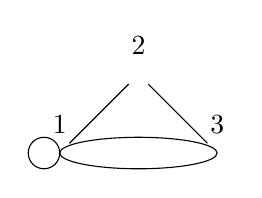
\begin{tikzpicture}
\filldraw 
(0,0) node[label=1](1){}
(1,1) node[label=2](2){} 
(2,0) node[label=3](3){};
\draw (0,0) arc (0:360:2mm);
\draw (2,0) arc (0:180:1 and 0.2);
\draw (0,0) arc (180:360:1 and 0.2);
\path[draw] (1)--(2);
\path[draw] (2)--(3);
\end{tikzpicture}
\captionsetup{justification=centering}
\caption{Przykład grafu~ogólnego} \label{fig:simple-graph}
\end{minipage}
\begin{minipage}{.45\textwidth}
  \centering
  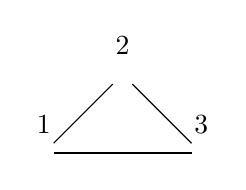
\begin{tikzpicture}
\filldraw 
(0,0) node[label=1](1){}
(1,1) node[label=2](2){} 
(2,0) node[label=3](3){};
\path[draw] (1)--(2);
\path[draw] (2)--(3);
\path[draw] (3)--(1);
\end{tikzpicture}
\captionsetup{justification=centering}
\caption{Przykład grafu~prostego} \label{fig:graph}
\end{minipage}
\end{figure}

\subsection*{Sąsiedztwo}

Wierzchołki $u,v \in V$ są \textbf{sąsiednie} jeśli istnieje krawędź $uv$ (wówczas wierzchołki $u$ i $v$ są \textbf{incydentne} z tą krawędzią). Dwie krawędzie są \textbf{sąsiednie}, jeśli są incydentne z tym samym wierzchołkiem. 

\textbf{Stopień} wierzchołka $v \in V$ jest liczbą krawędzi incydentnych z $v$. \textbf{Wierzchołek izolowany} to wierzchołek stopnia 0, a \textbf{wierzchołek końcowy} -- stopnia 1.

Istnieją dwie standardowe reprezentacje grafów w pamięci komputera: jako \textbf{listy sąsiedztwa} lub jako \textbf{macierze sąsiedztwa}\footcites[29]{banachowski}[600]{cormen}. Pierwsza z nich polega na zapamiętaniu dla każdego wierzchołka listy wierzchołków z nim sąsiadujących. Druga zakłada, że wierzchołki są ponumerowane liczbami ze zbioru $\{1, 2,\ldots,n\}$ (gdzie $n$ oznacza moc zbioru $V$) i opiera się na stworzeniu macierzy wymiaru $n \times n$, której wyraz o indeksach $i,j$ jest równy liczbie krawędzi łączących wierzchołek o numerze $i$ z wierzchołkiem o numerze $j$.

Innym sposobem reprezentacji grafu za pomocą macierzy jest \textbf{macierz incydencji}. Jeśli krawędzie oznakujemy liczbami ze zbioru $\{1,2,\ldots,m\}$ (gdzie $m$ moc zbioru $E$), to jest to macierz o rozmiarze $n \times m$, której wyraz o indeksach $i,j$ jest równy 1, jeśli wierzchołek z numerem $i$ jest incydentny z krawędzią $j$, i jest równy 0 w przeciwnym przypadku\footcite[27]{ross}.

\begin{figure}[H]
\centering
  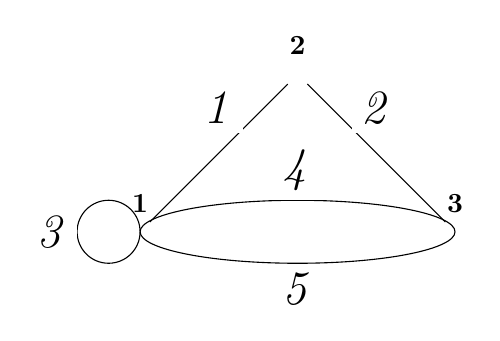
\begin{tikzpicture}
\filldraw 
(0,0) node[label=\textbf{1}](1){}
(2,2) node[label=\textbf{2}](2){} 
(4,0) node[label=\textbf{3}](3){};
\draw (0,0) arc (0:360:4mm) node [midway,left,fill=white] {\LARGE\textit{3}};
\draw (4,0) arc (0:180:2 and 0.4) node [midway,above,fill=white] {\LARGE\textit{4}};;
\draw (0,0) arc (180:360:2 and 0.4) node [midway,below,fill=white] {\LARGE\textit{5}};;
\path[draw] (1)--(2) node [midway,above=7pt,fill=white] {\LARGE\textit{1}};
\path[draw] (2)--(3) node [midway,above=7pt,fill=white] {\LARGE\textit{2}};
\end{tikzpicture}
\caption{}\label{fig:graph-edge-labeled}
\end{figure}

Macierz sąsiedztwa $A$ i macierz incydencji $M$ dla grafu z rysunku \ref{fig:graph-edge-labeled}:

\[A = 
 \begin{pmatrix}
  1 & 1 & 2 \\
  1 & 0 & 1 \\
  2 & 1 & 0 
 \end{pmatrix}, \hspace{20pt}
 M = 
 \begin{pmatrix}
  1 & 0 & 1 & 1 & 1 \\
  1 & 1 & 0 & 0 & 0 \\
  0 & 1 & 0 & 1 & 1 
 \end{pmatrix}
\]

\subsection*{Trasa, ścieżka, droga, cykl}

\textbf{Trasa} w grafie $G$ to skończony ciąg krawędzi $v_0v_1,v_1v_2\ldots v_{m-1}v_m$ (zapisywany również w postaci $v_0 \rightarrow v_1 \rightarrow \ldots \rightarrow v_m$), w którym każde dwie kolejne krawędzie są albo sąsiednie, albo identyczne\footcite[41]{wilson}. Trasa wyznacza ciąg wierzchołków $v_0,v_1,\ldots,v_m$ -- pierwszy z nich nazywamy \textbf{wierzchołkiem początkowym}, a ostatni \textbf{wierzchołkiem końcowym}. Liczba krawędzi na trasie to \textbf{długość trasy}. 

\textbf{Ścieżka} to trasa, w której wszystkie krawędzie są różne. Jeśli również wszystkie wierzchołki $v_0,v_1,\ldots,v_m$ są różne (dopuszczając jedynie możliwość, aby wierzchołek początkowy był równy wierzchołkowi końcowemu), to ścieżka nazywana jest \textbf{drogą}. Droga (lub ścieżka) jest \textbf{zamknięta}, jeśli $v_0 = v_m$; ścieżka zamknięta, która posiada co najmniej jedną krawędź to \textbf{cykl}; droga zamknięta, która posiada co najmniej jedną krawędź to \textbf{cykl prosty}.

Jeśli istnieje ścieżka z $u$ do $v$, to mówimy, że $v$ jest \textbf{osiągalny} z $u$.

\subsection*{Graf skierowany}

\textbf{Graf skierowany}, \textbf{digraf} (ang. \textit{directed graph}) $G$ to para $(V(G),\ E(G))$, gdzie $V(G)$ niepusty, skończony zbiór elementów zwanych \textbf{wierzchołkami}, a $E(G)$ skończony zbiór par \emph{uporządkowanych} elementów ze zbioru $V(G)$ zwanych \textbf{krawędziami} (lub \textbf{łukami}\footcite[135]{wilson}). Digraf $G$ jest \textbf{digrafem prostym}, jeśli wszystkie krawędzie są różne oraz jeśli nie posiada pętli. 

Jeśli $e = (v,w) \in E(G)$, to $v$ nazywamy \textbf{początkiem krawędzi} $e$, a $w$ -- \textbf{końcem krawędzi} $e$.

Definicje z poprzedniej podsekcji w naturalny sposób uogólniają się na przypadek digrafów\footcite[136]{wilson}. 

\subsection*{Spójność}

Załóżmy, że mamy dwa grafy $G_1 = (V_1,E_1)$ oraz $G_2 = (V_2,E_2)$, gdzie $V_1 \cap V_2 = \emptyset$. Wówczas \textbf{sumą} tych grafów $G_1 \cup G_2$ jest graf $G=(V_1\cup V_2, E_1\cup E_2)$. Graf nazywamy \textbf{spójnym}, jeśli nie można przedstawić go w postaci sumy dwóch grafów, w przeciwnym razie graf jest \textbf{niespójny}\footcite[22]{wilson}. Każdy graf niespójny $G$ możemy przedstawić jako sumę grafów spójnych, nazywanych \textbf{spójnymi składowymi} grafu $G$ (rysunek \ref{fig:connected-copoments-example} przedstawia graf posiadający dwie spójne składowe). 

\begin{figure}[h]
\centering
\begin{tikzpicture}
\filldraw 
(0,0) node(1){}
(1,1) node(2){} 
(2,0) node(3){}
(4,0) node(4){}
(4,1) node(5){};
\path[draw] (1)--(2);
\path[draw] (2)--(3);
\path[draw] (3)--(1);
\path[draw] (4)--(5);
\end{tikzpicture}
\caption{Przykład grafu mającego dwie spójne składowe} \label{fig:connected-copoments-example}
\end{figure}

Niektórzy autorzy\footcite[342]{ross} podają alternatywną, równoważną\footcite[42]{wilson} definicję grafu spójnego -- jest to graf, w którym każda para różnych wierzchołków jest połączona drogą. 

Graf skierowany $G$ jest \textbf{silnie spójny}, jeśli dla dowolnych dwóch wierzchołków $v$ i $w$ istnieje droga z $v$ do $w$. Każdy digraf silnie spójny jest spójny, ale nie wszystkie digrafy spójne są silnie spójne. 

\textbf{Dwuspójną składową} grafu $G$ nazywamy maksymalny podzbiór krawędzi, taki że każde dwie krawędzie z tego zbioru leżą na wspólnym cyklu prostym \footcite[634]{cormen}. W dwuspójnej składowej pomiędzy każdą parą wierzchołków istnieją dwie rozłączne krawędziowo drogi. Wierzchołki należące do co najmniej dwóch różnych dwuspójnych składowych nazywamy \textbf{wierzchołkami rozdzielającymi} (lub \textbf{punktami artykulacji}\footcite[633]{cormen}). Usunięcie wierzchołka rozdzielającego ,,rozspójnia'' graf. Krawędzie, które nie należą do żadnego cyklu prostego nazywamy \textbf{mostami}. Ich usunięcie również ,,rozspójnia'' graf.

Graf, który posiada tylko jedną dwuspójną składową nazywamy \textbf{grafem dwuspójnym}\footcite[232]{banachowski}.

\begin{figure}[h]
\centering
\begin{tikzpicture}
\fill[fill=light-gray] (1,0) -- (0,1) -- (1,2) -- (2,1);
\filldraw 
(1,0) node[color=gray](1){}
(0,1) node[color=gray](2){} 
(2,1) node(3){}
(1,2) node[color=gray](4){};
\path[draw,color=gray] (1)--(2);
\path[draw,color=gray] (2)--(3);
\path[draw,color=gray] (3)--(4);
\path[draw,color=gray] (4)--(1);
\path[draw,color=gray] (1)--(3);
\path[draw,color=gray] (2)--(4);

\fill[fill=light-gray] (5,0) -- (4,1) -- (5,2);
\filldraw 
(5,0) node[color=gray](5){}
(4,1) node(6){} 
(5,2) node[color=gray](7){};
\path[draw,color=gray] (5)--(6);
\path[draw,color=gray] (6)--(7);
\path[draw,color=gray] (7)--(5);
\path[draw] (3)--(6);
\end{tikzpicture}
\captionsetup{justification=centering}
\caption{Przykład grafu zawierającego trzy dwuspójne składowe -- punkty artykulacji i mosty zostały zaznaczone na czarno.} \label{fig:biconnected-copoments-example}
\end{figure}

\section{Przykłady grafów} \label{sec:common-graphs}

\subsection*{Graf pusty}

\textbf{Graf pusty} to graf, którego zbiór krawędzi jest zbiorem pustym. Każdy wierzchołek grafu pustego jest wierzchołkiem izolowanym. \blockquote{Grafy puste nie są zbyt interesujące}\footcite[30]{wilson}.

\begin{figure}[h]
\centering
\begin{tikzpicture}
\filldraw 
(0,1) node(1){}
(1,1) node(2){}
(1,2) node(3){}
(0,2) node(4){};
\end{tikzpicture}
\captionsetup{justification=centering}
\caption{Przykład grafu pustego mającego cztery wierzchołki} \label{fig:empty-graph-example}
\end{figure}

\subsection*{Graf pełny}

\textbf{Graf pełny} to graf prosty, którego każda para różnych wierzchołków jest połączona krawędzią. Graf pełny mający $n$ wierzchołków oznacza się symbolem $K_n$. 

\begin{figure}[h]
\centering

\begin{tikzpicture}
\filldraw 
(0,1) node(1){}
(1,1) node(2){}
(1,2) node(3){}
(0,2) node(4){};
\path[draw,color=gray] (1)--(2);
\path[draw,color=gray] (1)--(3);
\path[draw,color=gray] (1)--(4);
\path[draw,color=gray] (2)--(3);
\path[draw,color=gray] (2)--(4);
\path[draw,color=gray] (3)--(4); 
\end{tikzpicture}
\captionsetup{justification=centering}
\caption{Przykład grafu $K_4$} \label{fig:complete-graph-example}
\end{figure}

\subsection*{Graf regularny}

\textbf{Graf regularny} to graf, w którym każdy wierzchołek ma ten sam stopień. Jeśli każdy wierzchołek ma stopień $r$, to graf nazywa się \textbf{grafem regularnym stopnia $r$} (lub \textbf{grafem $r$-regularnym})\footcite[31]{wilson}. Przykładem grafu regularnego stopnia 3 jest \textbf{graf Petersena} przedstawiony na rysunku \ref{fig:petersen-graph}. Każdy graf pusty jest grafem $0$-regularnym, a graf pełny $K_n$ jest grafem regularnym stopnia $n-1$. 

\begin{figure}[h]
\centering
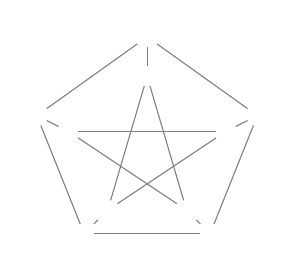
\begin{tikzpicture}
\filldraw 
(1,1.5) node(1){}
(1.5,0.5) node(2){}
(2,2.2) node(3){}
(2.5,0.5) node(4){}
(3,1.5) node(5){}%
(0.6,1.7) node(6){}
(1.2,0.2) node(7){}
(2,2.7) node(8){}
(2.8,0.2) node(9){}
(3.4,1.7) node(10){};
\path[draw,color=gray] (1)--(4);
\path[draw,color=gray] (1)--(5);
\path[draw,color=gray] (2)--(3);
\path[draw,color=gray] (2)--(5);
\path[draw,color=gray] (3)--(4);
\path[draw,color=gray] (6)--(1);
\path[draw,color=gray] (6)--(7);
\path[draw,color=gray] (6)--(8);
\path[draw,color=gray] (8)--(3);
\path[draw,color=gray] (8)--(10);
\path[draw,color=gray] (7)--(9);
\path[draw,color=gray] (7)--(2);
\path[draw,color=gray] (9)--(10);
\path[draw,color=gray] (9)--(4);
\path[draw,color=gray] (10)--(5);
\end{tikzpicture}
\captionsetup{justification=centering}
\caption{Graf Petersena} \label{fig:petersen-graph}
\end{figure}

\subsection*{Graf cykliczny, graf liniowy, koło}

\textbf{Graf cykliczny} to spójny graf regularny stopnia 2. Graf cykliczny mający $n$ wierzchołków oznacza się symbolem $C_n$. Graf liniowy o $n$ wierzchołkach (oznaczany symbolem $P_n$) to graf powstały przez usunięcie jednej krawędzi z $C_n$. tbc

\begin{figure}[h]
\centering
\begin{tikzpicture}
\filldraw 
(0,1) node(1){}
(1,1) node(2){}
(1,2) node(3){}
(0,2) node(4){};
\path[draw,color=gray] (1)--(2);
\path[draw,color=gray] (1)--(4);
\path[draw,color=gray] (2)--(3);
\path[draw,color=gray] (3)--(4); 
\end{tikzpicture}
\captionsetup{justification=centering}
\caption{Przykład grafu $C_4$} \label{fig:cycle-graph-example}
\end{figure}

\section{Zastosowania grafów}